% Repository:  https://github.com/chiehrosswang/TRB_LaTeX_tex
%
% Transportation Research Board conference paper template
% version 4.0 Lite (updates made to be compatible in Overleaf and ShareLaTeX)
%
%
% When numbered option is activated, lines are numbered.
\documentclass[numbered]{trbunofficial}
\usepackage{graphicx}
\usepackage{booktabs}

\newread\somefile
\usepackage{xparse}
\usepackage{natbib}
\bibliographystyle{unsrtnat}
\setcitestyle{round}
% \usepackage[colorlinks=true,linkcolor=blue,citecolor=blue]{hyperref}
% For TRB version hide links
\usepackage[hidelinks]{hyperref}

% Put here what will go to headers as author
\AuthorHeaders{Reynolds and Currie}
\title{Leveraging GTFS data to calculate an open-source Transit Supply
Index}

% TODO: add macros for easier formatting of \author.
\author{%
    \textbf{James Reynolds}\\\textit{Corresponding Author}\\
  Research Fellow\\
  Public Transport Research Group, Institute of Transport Studies,
Department of Civil Engineering, Monash University, Victoria,
Australia\\
  \href{mailto:james.reynolds@monash.edu}{\nolinkurl{james.reynolds@monash.edu}}\\
  \hfill\break
    \textbf{Graham Currie}\\
  Professor\\
  Public Transport Research Group, Institute of Transport Studies,
Department of Civil Engineering, Monash University, Victoria,
Australia\\
  \href{mailto:graham.currie@monash.edu}{\nolinkurl{graham.currie@monash.edu}}\\
  \hfill\break
  }

% If necessary modify the number of words per table or figure default is set to
% 250 words per table (default defined in cls)


% If words are counted manually, put that number here. This does not include
% figures and tables. This can also be used to avoid problems with texcount
% program i.e. if one does not have it installed.
\TotalWords{684}


% tightlist command for lists without linebreak
\providecommand{\tightlist}{%
  \setlength{\itemsep}{0pt}\setlength{\parskip}{0pt}}




\begin{document}
\maketitle


\section{Abstract}
TBC.
\hfill\break%
\hfill\break%
\noindent\textit{Keywords}:  Transit, Public
transport, GTFS, Benchmarking,  
\newpage

\hypertarget{introduction}{%
\section{Introduction}\label{introduction}}

Transit service level indicators include those in the Transit Capacity
and Quality of Service Manual (TCQSM) \citep{TCQSM:2013}, the Transit
Score metric and many more. Practitioners, researchers and advocates
seeking to use such metrics may face two inter-related challenges:
firstly, there is the problem of calculating the metrics themselves for
a specific location; secondly, is the challenge of explaining the
metrics, their meaning and importance those who are not specialists in
transit, such as politicians, other decision-makers or the general
public.

The TCQSM specifies Levels of Service (LOS) between A and F across a
range of factors including service span, frequency, speed, and the
proportion of population serviced. Previous research by
\citet{Wong:2013aa} overcame some challenges of using the TCQSM, by
using Python, PostgreSQL and R software and GTFS feeds as input to
automate the calculation of daily average headways, route length and
stop numbers. This indicators, however, are route based and so do not
include any consideration of geographic or population coverage. Further
metrics addressing these topics and much detail about their calculation
and meaning are included in the TCQSM, such as the Service Coverage Area
(pp.~5-8 to 5-21). However, these appear highly detailed, may required
bespoke GIS or other analysis, and it might be challenging to explain
these measures (beyond the fact at A is good and F is bad) to
non-technical decision-makers, stakeholders or others who might be
involved. Transit Score provides a similarly easily understood rating
scale, scoring locations out of 100 \citep{WalkScore:2023tg}. However,
the algorithm is patented and effectively a black box, meaning that it
is not possible to calculate scores independently to understand how the
metric might change with cahnges to the transit system or surrounding
environment.

The Supply Index developed by \citet{currie2007identifying} may provide
a metric that is relatively easy to calculate, open (rather than a black
box), and relatively simple for a non-technical audience to understand,
engage with and use. This Index is based on calculating the number of
transit arrivals at stops within an area of interest, with an adjustment
made for the amount of the area of interest that is within a typical
walk access distance of each stop. However, it does not appear to have
been widely used, perhaps in part because it still required an analyst
to obtain sources of timetable and geographic data. Since the
publication of \citet{currie2007identifying} such data has become much
easier to obtain with more than 10,000 agencies now providing timetable
and network data using the General Transit Feed Specification (GTFS)
format \citep{GTFS}. A gap, however, is that there is not yet a method
for calculating the \citet{currie2007identifying} Supply Index directly
from GTFS data.

This paper reports the development of R code to calculate the Supply
Index of \citet{currie2007identifying} directly from GTFS data. The code
is developed using data from a single case: the GTFS for Victoria in
Australia, which includes Greater Melbourne. Cross-case comparison to
Toronto, Canada, and Washington DC, USA, is also undertaken to test the
results and gain understanding of how the Supply Index might be useful
for practitioners, researchers and advocates. The motivation for this
research is to better understand how GTFS data might be used to produce
benchmarking metrics that can be calculated using open-source code, that
can be used to access proposed network changes and which may be
relatively easy for non-technical specialists to understand.

\hypertarget{research-context}{%
\section{Research context}\label{research-context}}

Even a brief search shows that there is a very large number of metrics
available for benchmarking transit services, for example: the Transit
Cooperative Research Program (TCRP) Report 88 provides an extensive
guidebook on developing a performance-measurement system
\citep{Ryus:2003aa}; online databases are provided by the Florida
Transit Information System (FTIS)
\citep{Florida-Transit-Information-System:2018aa} and the International
Association of Public Transport (UITP) \citep{UITP:2015aa} have online
databases, while the Transport Strategy Centre of Imperial College
London runs extensive annual benchmarking programmes across over 100
transit provides around the world
\citep{Imperial-College-London:2023aa}.

The TCQSM and Transit Score may provide contrasting examples: with
respect to the first challenge, TCQSM metrics may require large amounts
of network, service, population and other data to be assembled before
the indicators can be calculated; whereas Transit Scores are readily
available on the \citet{WalkScore:2023tg} website for locations with a
published GTFS feed (eliminating the need for any calculations). With
respect to the second challenge, the meaning of the Transit Score
appears easy to explain (the closer to 100, the better), but as the
score is calculated by a patented algorithm (effectively a black-box) it
may not be easy to understand or explain the connection between
real-world conditions and the score, or what might need to be done to
improve the score and service levels. Nor does it appear to be possible
for Transit Scores to be generated for proposed changes to networks. The
TCQSM, in

\hypertarget{general-transit-feed-specification-gtfs}{%
\subsection{General Transit Feed Specification
(GTFS)}\label{general-transit-feed-specification-gtfs}}

\hypertarget{social-needs-and-the-suppy-index}{%
\subsection{Social needs and the Suppy
Index}\label{social-needs-and-the-suppy-index}}

\footnote{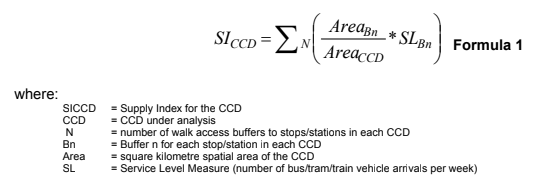
\includegraphics{Supply_index.png}}

he SI\textsubscript{CCD} can then be compared between different CCDs to
give an indication of the relative supply of transit, adjusted for
accessibility.

An advantage of the Supply Index is that it is a relatively simple
number to calculate, understand and explain. It is based on the number
of bus/tram/train arrivals per week at stops within the CCD, which is
multiplied by a factor allowing for the amount of the CCD that is within
walking distance of each stop \footnote{This is the
  Area\textsubscript{Bn} divided by Area\textsubscript{CCD} part of the
  calculation. Thresholds for access of 400m for bus and tram stops, and
  800m for railway stations are used in the calculation of the
  Area\textsubscript{Bn} variable.}.

\citet{currie2007identifying} calculated the SI for various CCDs in
Melbourne using a timetable database provided by the Victorian Public
Transport Authority (PTA). This predated the widespread availability of
GTFS data, which provides a standardised format for timetable data that
is produced by many transit systems. A question, therefore, is how to
calculate the SI using GTFS data so that SI\textsubscript{CCD}s can be
calculated for current services in Melbourne or other places.

\hypertarget{methodology}{%
\section{Methodology}\label{methodology}}

\hypertarget{results}{%
\section{Results}\label{results}}

\hypertarget{r-code}{%
\subsection{R code}\label{r-code}}

\hypertarget{case-studies}{%
\subsection{Case studies}\label{case-studies}}

\hypertarget{melbourne}{%
\subsubsection{Melbourne}\label{melbourne}}

Overall

Wheelchair accessibility?

The metro tunnel - adding services

\hypertarget{toronto}{%
\subsubsection{Toronto}\label{toronto}}

\hypertarget{washington-dc}{%
\subsubsection{Washington DC}\label{washington-dc}}

\hypertarget{cross-case-comparison}{%
\subsubsection{Cross-case comparison}\label{cross-case-comparison}}

\hypertarget{discussion}{%
\section{Discussion}\label{discussion}}

\hypertarget{conclusions}{%
\section{Conclusions}\label{conclusions}}

\hypertarget{author-contribution-statement}{%
\section{Author Contribution
Statement}\label{author-contribution-statement}}

The authors confirm contribution to the paper as follows: study
conception and design: A. Anonymous, D. Zoolander; data collection: B.
Security; analysis and interpretation of results: A. Anonymous, B.
Security; draft manuscript preparation: A. Anonymous. All authors
reviewed the results and approved the final version of the manuscript.

\hypertarget{acknowledgements}{%
\section{Acknowledgements}\label{acknowledgements}}

This document was prepared using the \texttt{rticles} template, created
by Gregory Macfarlane, which is based on the \LaTeX originally posted by
David Pritchard in 2009 and updated it in 2011, soon after TRB began
allowing PDF submissions. Gregory Macfarlane and Ross Wang made
adjustments to the template, and Ross Wang now maintains the
\LaTeX template at \url{https://github.com/chiehrosswang/TRB_LaTeX_tex}.
Gregory Macfarlane created the \texttt{rticles} template in 2021.

\newpage
\renewcommand\refname{References}
\bibliography{packages.bib,References.bib}


\end{document}
